\section{Phần 1: Lý Thuyết Data Fitting và Minh Họa}

Phần này trình bày nền tảng toán học của bài toán Data Fitting và phương pháp
Ordinary Least Squares (OLS), kèm theo cài đặt Python từ đầu để minh họa và
kiểm chứng từng kết quả lý thuyết.

% ------------------------------------------------------------
\subsection{Bài Toán Data Fitting}
% ------------------------------------------------------------

\subsubsection{Phát Biểu Bài Toán Tổng Quát}

\begin{tcolorbox}[mycodebox, colback=blue!3!white, colframe=blue!40!black,
    title={\textbf{Định nghĩa 1.1} - Bài Toán Data Fitting}]
Cho tập dữ liệu $\mathcal{D} = \{(\mathbf{x}_i, y_i)\}_{i=1}^n$ với
$\mathbf{x}_i \in \mathbb{R}^p$, $y_i \in \mathbb{R}$.
Bài toán Data Fitting là tìm hàm $f : \mathbb{R}^p \to \mathbb{R}$ trong một
lớp hàm cho trước sao cho $f$ xấp xỉ tốt nhất ánh xạ từ $\mathbf{x}_i$ đến
$y_i$ theo một tiêu chí đã định.
\end{tcolorbox}

Trong mô hình \textbf{hồi quy tuyến tính}, ta giả thiết quan hệ tuyến tính
giữa các biến độc lập và biến phụ thuộc:
\begin{equation}
    y_i = \beta_0 + \beta_1 x_{i1} + \beta_2 x_{i2} + \cdots + \beta_p x_{ip}
          + \epsilon_i
        = \mathbf{x}_i^T \boldsymbol{\beta} + \epsilon_i,
    \label{eq:linear_model}
\end{equation}
với $\boldsymbol{\beta} = (\beta_0, \beta_1, \ldots, \beta_p)^T \in \mathbb{R}^{p+1}$
là vector tham số cần ước lượng và $\epsilon_i$ là nhiễu ngẫu nhiên.

Viết dưới dạng ma trận, với
$\mathbf{X} \in \mathbb{R}^{n \times (p+1)}$ là \emph{ma trận design} (cột đầu
toàn 1 đại diện cho intercept):
\begin{equation}
    \mathbf{y} = \mathbf{X}\boldsymbol{\beta} + \boldsymbol{\varepsilon},
    \label{eq:matrix_form}
\end{equation}
trong đó $\mathbf{y} \in \mathbb{R}^n$ là vector quan sát và
$\boldsymbol{\varepsilon} \in \mathbb{R}^n$ là vector nhiễu.

\subsubsection{Các Giả Thiết Gauss–Markov}

Để đảm bảo OLS có các tính chất tốt, ta cần các giả thiết Gauss–Markov
(GM1–GM5):

\begin{enumerate}[label=\textbf{GM\arabic*.}]
    \item \textbf{Tuyến tính:} $\mathbf{y} = \mathbf{X}\boldsymbol{\beta} +
          \boldsymbol{\varepsilon}$.
    \item \textbf{Không hoàn hảo đa cộng tuyến:} $\rank(\mathbf{X}) = p+1$
          (các cột của $\mathbf{X}$ độc lập tuyến tính, đảm bảo
          $\mathbf{X}^T\mathbf{X}$ khả nghịch).
    \item \textbf{Ngoại sinh:} $E[\boldsymbol{\varepsilon} \mid \mathbf{X}] =
          \mathbf{0}$, tức $E[\epsilon_i \mid \mathbf{x}_i] = 0$ với mọi $i$.
    \item \textbf{Đồng phương sai (Homoscedasticity):}
          $\mathrm{Var}(\boldsymbol{\varepsilon} \mid \mathbf{X}) =
          \sigma^2 \mathbf{I}_n$, tức các sai số có cùng phương sai $\sigma^2$
          và không tương quan với nhau.
    \item \textbf{Phân phối chuẩn (tùy chọn):}
          $\boldsymbol{\varepsilon} \mid \mathbf{X} \sim
          \mathcal{N}(\mathbf{0}, \sigma^2 \mathbf{I}_n)$
          (cần cho kiểm định giả thuyết).
\end{enumerate}

% ------------------------------------------------------------
\subsection{Phương Pháp Ordinary Least Squares (OLS)}
% ------------------------------------------------------------

\subsubsection{Hàm Mất Mát và Nghiệm OLS}

OLS tìm $\hat{\boldsymbol{\beta}}$ tối thiểu hóa \emph{Tổng Bình Phương Phần
Dư} (Residual Sum of Squares - RSS):
\begin{equation}
    \mathrm{RSS}(\boldsymbol{\beta})
    = \|\mathbf{y} - \mathbf{X}\boldsymbol{\beta}\|_2^2
    = \sum_{i=1}^n (y_i - \mathbf{x}_i^T\boldsymbol{\beta})^2.
    \label{eq:rss}
\end{equation}

\begin{tcolorbox}[mycodebox, colback=blue!3!white, colframe=blue!40!black,
    title={\textbf{Định lý 1.1} - Nghiệm OLS (Normal Equations)}]
Nếu $\mathbf{X}^T\mathbf{X}$ khả nghịch, nghiệm OLS duy nhất là:
\begin{equation}
    \hat{\boldsymbol{\beta}}_{\mathrm{OLS}}
    = (\mathbf{X}^T\mathbf{X})^{-1}\mathbf{X}^T\mathbf{y}.
    \label{eq:ols_solution}
\end{equation}
\end{tcolorbox}

\textbf{Chứng minh.} Lấy đạo hàm của RSS theo $\boldsymbol{\beta}$:
\begin{align}
    \nabla_{\boldsymbol{\beta}}\,\mathrm{RSS}
    &= \nabla_{\boldsymbol{\beta}}
       \bigl[(\mathbf{y} - \mathbf{X}\boldsymbol{\beta})^T
             (\mathbf{y} - \mathbf{X}\boldsymbol{\beta})\bigr] \notag \\
    &= -2\,\mathbf{X}^T(\mathbf{y} - \mathbf{X}\boldsymbol{\beta}).
\end{align}
Cho đạo hàm bằng $\mathbf{0}$:
$\mathbf{X}^T\mathbf{X}\boldsymbol{\beta} = \mathbf{X}^T\mathbf{y}$
(phương trình pháp tuyến - \emph{Normal Equations}).
Vì $\mathbf{X}^T\mathbf{X}$ khả nghịch (theo GM2), suy ra
$\hat{\boldsymbol{\beta}} = (\mathbf{X}^T\mathbf{X})^{-1}\mathbf{X}^T\mathbf{y}$.
Để kiểm tra đây là cực tiểu (không phải cực đại), ta kiểm tra đạo hàm bậc 2:
$\nabla^2_{\boldsymbol{\beta}}\,\mathrm{RSS} = 2\mathbf{X}^T\mathbf{X}$
là ma trận xác định dương (positive definite) vì $\rank(\mathbf{X}) = p+1$.
$\hfill\square$

\textbf{Cài đặt Python - F1: \texttt{ols\_fit}:}

\begin{lstlisting}[language=Python, caption={Hàm \texttt{ols\_fit} - tính nghiệm OLS từ công thức Normal Equations}]
def ols_fit(X: list[list[float]], y: list[float]) -> dict:
    """F1: Tinh beta_hat = (X^T X)^{-1} X^T y va sigma2_hat."""
    n, p = len(X), len(X[0])
    X_b  = add_bias(X)                        # them cot 1 (intercept)
    Xt   = transpose(X_b)                     # utils.py
    XtX  = matmul(Xt, X_b)                    # utils.py
    Xty  = matvec(Xt, y)                      # utils.py
    beta_hat  = solve_system(XtX, Xty)        # utils.py (Gauss elim.)
    y_hat     = matvec(X_b, beta_hat)
    residuals = [y[i] - y_hat[i] for i in range(n)]
    rss       = sum(r * r for r in residuals)
    sigma2    = rss / max(n - p - 1, 1)       # ung luong khong chech
    return {"beta_hat": beta_hat, "sigma2_hat": sigma2,
            "y_hat": y_hat, "residuals": residuals}
\end{lstlisting}

Hàm \texttt{solve\_system} trong \texttt{utils.py} giải hệ $\mathbf{A}\mathbf{x}
= \mathbf{b}$ bằng phép khử Gauss với partial pivoting, tránh sử dụng
\texttt{numpy.linalg.solve} đúng theo yêu cầu đề bài.

\subsubsection{Ma Trận Chiếu và Hat Matrix}

\begin{tcolorbox}[mycodebox, colback=blue!3!white, colframe=blue!40!black,
    title={\textbf{Định nghĩa 1.2} - Hat Matrix}]
Ma trận chiếu (projection matrix) hay \emph{Hat Matrix} được định nghĩa:
\begin{equation}
    \mathbf{H} = \mathbf{X}(\mathbf{X}^T\mathbf{X})^{-1}\mathbf{X}^T
    \in \mathbb{R}^{n \times n}.
    \label{eq:hat_matrix}
\end{equation}
\end{tcolorbox}

Tên ``Hat Matrix'' xuất phát từ tính chất $\hat{\mathbf{y}} = \mathbf{H}\mathbf{y}$
- ma trận ``đội mũ'' lên $\mathbf{y}$ để tạo ra giá trị dự đoán $\hat{\mathbf{y}}$.

\begin{tcolorbox}[mycodebox, colback=green!3!white, colframe=green!40!black,
    title={\textbf{Mệnh đề 1.1} - Tính Chất của $\mathbf{H}$}]
\begin{enumerate}[label=(\roman*)]
    \item $\mathbf{H}^2 = \mathbf{H}$ \hfill (idempotent - lũy đẳng)
    \item $\mathbf{H}^T = \mathbf{H}$ \hfill (đối xứng)
    \item Giá trị riêng của $\mathbf{H}$: chỉ là $0$ hoặc $1$
    \item $\rank(\mathbf{H}) = \mathrm{tr}(\mathbf{H}) = p+1$
    \item $\hat{\mathbf{y}} = \mathbf{H}\mathbf{y}$;\quad
          $\hat{\boldsymbol{\varepsilon}} = (\mathbf{I} - \mathbf{H})\mathbf{y}$
    \item $(\mathbf{I}-\mathbf{H})$ cũng idempotent và đối xứng
\end{enumerate}
\end{tcolorbox}

\textbf{Chứng minh các tính chất.}
\begin{itemize}
    \item \textit{(i) Idempotent:}
    $\mathbf{H}^2 = \mathbf{X}(\mathbf{X}^T\mathbf{X})^{-1}\mathbf{X}^T
                   \mathbf{X}(\mathbf{X}^T\mathbf{X})^{-1}\mathbf{X}^T
               = \mathbf{X}(\mathbf{X}^T\mathbf{X})^{-1}\mathbf{X}^T = \mathbf{H}$.
    \item \textit{(ii) Đối xứng:}
    $\mathbf{H}^T = \bigl[\mathbf{X}(\mathbf{X}^T\mathbf{X})^{-1}\mathbf{X}^T\bigr]^T
               = \mathbf{X}\bigl[(\mathbf{X}^T\mathbf{X})^{-1}\bigr]^T\mathbf{X}^T
               = \mathbf{X}(\mathbf{X}^T\mathbf{X})^{-1}\mathbf{X}^T = \mathbf{H}$
    (vì $(\mathbf{X}^T\mathbf{X})$ đối xứng nên nghịch đảo cũng đối xứng).
    \item \textit{(iii) Giá trị riêng:} Nếu $\lambda$ là giá trị riêng của $\mathbf{H}$,
    từ $\mathbf{H}^2 = \mathbf{H}$ suy ra $\lambda^2 = \lambda$, tức $\lambda \in \{0, 1\}$.
    \item \textit{(iv) Rank:} Vì $\mathbf{H}$ idempotent,
    $\rank(\mathbf{H}) = \mathrm{tr}(\mathbf{H})
    = \mathrm{tr}\bigl[\mathbf{X}(\mathbf{X}^T\mathbf{X})^{-1}\mathbf{X}^T\bigr]
    = \mathrm{tr}\bigl[(\mathbf{X}^T\mathbf{X})^{-1}\mathbf{X}^T\mathbf{X}\bigr]
    = \mathrm{tr}(\mathbf{I}_{p+1}) = p+1$.
\end{itemize}

\subsubsection{Định Lý Gauss–Markov}

\begin{tcolorbox}[mycodebox, colback=blue!3!white, colframe=blue!40!black,
    title={\textbf{Định lý 1.2} - Gauss–Markov (BLUE)}]
Dưới các giả thiết GM1–GM4, ước lượng OLS
$\hat{\boldsymbol{\beta}}_{\mathrm{OLS}}$ là ước lượng tuyến tính không
chệch tốt nhất (\emph{Best Linear Unbiased Estimator} - \textbf{BLUE}):
\begin{enumerate}[label=(\roman*)]
    \item \textbf{Không chệch (Unbiased):}
          $E[\hat{\boldsymbol{\beta}}_{\mathrm{OLS}}] = \boldsymbol{\beta}$.
    \item \textbf{Tốt nhất (Best):} Với mọi ước lượng tuyến tính không chệch
          $\tilde{\boldsymbol{\beta}}$ khác,
          $\mathrm{Var}(\tilde{\beta}_j) \geq \mathrm{Var}(\hat{\beta}_j^{\mathrm{OLS}})$
          với mọi $j$.
\end{enumerate}
Ma trận hiệp phương sai của $\hat{\boldsymbol{\beta}}_{\mathrm{OLS}}$:
\begin{equation}
    \mathrm{Var}(\hat{\boldsymbol{\beta}}_{\mathrm{OLS}} \mid \mathbf{X})
    = \sigma^2(\mathbf{X}^T\mathbf{X})^{-1}.
    \label{eq:var_beta}
\end{equation}
\end{tcolorbox}

\textbf{Chứng minh tính không chệch.}
\begin{align}
    E[\hat{\boldsymbol{\beta}}_{\mathrm{OLS}}]
    &= E\bigl[(\mathbf{X}^T\mathbf{X})^{-1}\mathbf{X}^T\mathbf{y}\bigr] \notag \\
    &= (\mathbf{X}^T\mathbf{X})^{-1}\mathbf{X}^T
       E[\mathbf{X}\boldsymbol{\beta} + \boldsymbol{\varepsilon}] \notag \\
    &= (\mathbf{X}^T\mathbf{X})^{-1}\mathbf{X}^T\mathbf{X}\boldsymbol{\beta}
       + (\mathbf{X}^T\mathbf{X})^{-1}\mathbf{X}^T
         \underbrace{E[\boldsymbol{\varepsilon} \mid \mathbf{X}]}_{=\mathbf{0}\text{ (GM3)}}
    = \boldsymbol{\beta}. \quad \square
\end{align}

\textbf{Chứng minh ma trận hiệp phương sai.}
\begin{align}
    \mathrm{Var}(\hat{\boldsymbol{\beta}})
    &= \mathrm{Var}\bigl[(\mathbf{X}^T\mathbf{X})^{-1}\mathbf{X}^T\mathbf{y}\bigr]
     = (\mathbf{X}^T\mathbf{X})^{-1}\mathbf{X}^T
       \underbrace{\mathrm{Var}(\mathbf{y})}_{=\sigma^2\mathbf{I}_n}
       \mathbf{X}(\mathbf{X}^T\mathbf{X})^{-1}
     = \sigma^2(\mathbf{X}^T\mathbf{X})^{-1}. \quad \square
\end{align}

\textbf{Minh họa Monte Carlo - Định lý Gauss–Markov (F10):}

Để kiểm chứng định lý bằng mô phỏng, ta thực hiện $N_{\mathrm{sim}} = 1000$
lần với cùng ma trận $\mathbf{X}$ cố định, mỗi lần sinh ngẫu nhiên
$\boldsymbol{\varepsilon} \sim \mathcal{N}(\mathbf{0}, \sigma^2\mathbf{I})$
và tính $\hat{\boldsymbol{\beta}}_{\mathrm{OLS}}$. Bên cạnh đó, xây dựng
estimator thay thế $\tilde{\boldsymbol{\beta}} = \hat{\boldsymbol{\beta}} +
c\,\mathbf{e}_0 (\mathbf{v}^T\mathbf{y})$ với
$\mathbf{v} \in \mathrm{Null}(\mathbf{X}^T)$
(vẫn là ước lượng không chệch nhưng có phương sai lớn hơn).

Trước khi quay lại phần cài đặt, Hình~\ref{fig:gauss_markov} đóng vai trò như một kiểm chứng
thực nghiệm cho phần chứng minh ở trên: nếu các giả định Gauss--Markov được giữ, OLS không chỉ
không chệch mà còn có phương sai nhỏ nhất trong lớp ước lượng tuyến tính không chệch được thử.
Kết quả mô phỏng xác nhận:
\begin{itemize}
    \item $E[\hat{\boldsymbol{\beta}}_{\mathrm{OLS}}] \approx \boldsymbol{\beta}$
          (sai số trung bình $< 0.01$).
    \item $\mathrm{Var}(\hat{\beta}_j^{\mathrm{OLS}}) \leq
          \mathrm{Var}(\tilde{\beta}_j)$ với mọi $j$.
\end{itemize}

\begin{figure}[h]
    \centering
    
\includegraphics[width=0.92\textwidth]{assets/part1/gauss_markov_histograms.png}
    \caption{Phân phối $\hat{\boldsymbol{\beta}}_{\mathrm{OLS}}$ (xanh) và
             $\tilde{\boldsymbol{\beta}}_{\mathrm{alt}}$ (cam) qua 1000 mô phỏng.
             Đường đỏ dọc là giá trị $\beta$ thực.
             OLS tập trung xung quanh $\beta$ thực (không chệch) với độ phân
             tán thấp hơn estimator thay thế (phương sai nhỏ hơn).}
    \label{fig:gauss_markov}
\end{figure}

\subsubsection{Ước Lượng Phương Sai Nhiễu}

\begin{tcolorbox}[mycodebox, colback=green!3!white, colframe=green!40!black,
    title={\textbf{Định lý 1.3} - Ước Lượng Không Chệch của $\sigma^2$}]
\begin{equation}
    \hat{\sigma}^2
    = \frac{\mathrm{RSS}}{n - p - 1}
    = \frac{\|\mathbf{y} - \mathbf{X}\hat{\boldsymbol{\beta}}\|^2}{n - p - 1},
    \label{eq:sigma2}
\end{equation}
với $n - p - 1$ là bậc tự do còn lại sau khi ước lượng $p+1$ tham số.
Ta có $E[\hat{\sigma}^2] = \sigma^2$.
\end{tcolorbox}

\textbf{Lưu ý triển khai:} Hàm \texttt{ols\_fit} tính $\hat{\sigma}^2$
sử dụng \texttt{n - p - 1} bậc tự do (không phải $n - 2$),
đảm bảo tính đúng khi số biến $p > 1$.

% ------------------------------------------------------------
\subsection{Đánh Giá Mô Hình}
% ------------------------------------------------------------

\subsubsection{Hệ Số Xác Định $R^2$ và $\bar{R}^2$ Hiệu Chỉnh}

Phân rã tổng bình phương (ANOVA decomposition):
\begin{equation}
    \underbrace{\sum_i (y_i - \bar{y})^2}_{\mathrm{TSS}}
    = \underbrace{\sum_i (\hat{y}_i - \bar{y})^2}_{\mathrm{MSS}}
    + \underbrace{\sum_i (y_i - \hat{y}_i)^2}_{\mathrm{RSS}},
\end{equation}
với TSS (Total Sum of Squares), MSS (Model Sum of Squares) và RSS
(Residual Sum of Squares).

\begin{tcolorbox}[mycodebox, colback=blue!3!white, colframe=blue!40!black,
    title={\textbf{Định nghĩa 1.3} - Hệ Số Xác Định}]
\begin{align}
    R^2 &= 1 - \frac{\mathrm{RSS}}{\mathrm{TSS}}
         = \frac{\mathrm{MSS}}{\mathrm{TSS}} \in [0, 1],
    \label{eq:r2} \\
    \bar{R}^2 &= 1 - \frac{n-1}{n-p-1}(1 - R^2)
               = 1 - \frac{\mathrm{RSS}/(n-p-1)}{\mathrm{TSS}/(n-1)}.
    \label{eq:r2_adj}
\end{align}
\end{tcolorbox}

$R^2$ đo tỉ lệ phương sai của $y$ được giải thích bởi mô hình. Tuy nhiên,
$R^2$ luôn tăng khi thêm biến (kể cả biến không có ý nghĩa), do đó ta dùng
$\bar{R}^2$ để so sánh các mô hình có số biến khác nhau - $\bar{R}^2$ phạt
thêm biến thông qua hệ số $(n-1)/(n-p-1) > 1$.

\subsubsection{Kiểm Định Giả Thuyết}

Dưới giả thiết chuẩn GM5, ta có
$\hat{\boldsymbol{\beta}} \sim \mathcal{N}(\boldsymbol{\beta},\,
\sigma^2(\mathbf{X}^T\mathbf{X})^{-1})$.

\medskip
\noindent\textbf{Kiểm Định Student ($t$-test)} - kiểm định ý nghĩa của
từng hệ số $\beta_j$:
\begin{equation}
    t_j = \frac{\hat{\beta}_j}{\hat{\sigma}\sqrt{[(\mathbf{X}^T\mathbf{X})^{-1}]_{jj}}}
        \sim t_{n-p-1}
    \quad (H_0 : \beta_j = 0).
    \label{eq:t_test}
\end{equation}
Nếu $|t_j| > t_{n-p-1, \alpha/2}$ hoặc p-value $< \alpha$, ta bác bỏ $H_0$.

\medskip
\noindent\textbf{Kiểm Định F} - kiểm định ý nghĩa tổng thể của mô hình:
\begin{equation}
    F = \frac{\mathrm{MSS}/p}{\mathrm{RSS}/(n-p-1)}
      \sim F_{p,\, n-p-1}
    \quad (H_0 : \beta_1 = \cdots = \beta_p = 0).
    \label{eq:f_test}
\end{equation}

\textbf{Cài đặt Python - F4: \texttt{coef\_inference}:}

\begin{lstlisting}[language=Python, caption={Hàm \texttt{coef\_inference} - tính standard error, t-statistic, p-value và khoảng tin cậy 95\%}]
def coef_inference(X, y, beta_hat, sigma2) -> dict:
    """F4: SE, t-stat, p-value, CI 95% cho tung he so."""
    import math
    n, p = len(X), len(X[0])
    X_b  = add_bias(X)
    XtX_inv = inverse(matmul(transpose(X_b), X_b))  # utils.py
    se   = [math.sqrt(sigma2 * XtX_inv[j][j]) for j in range(p + 1)]
    t_stats = [beta_hat[j] / se[j] if se[j] > EPSILON else 0.0
               for j in range(p + 1)]
    # p-value (two-tailed) tu phan phoi t_{n-p-1}
    df   = n - p - 1
    p_values = [2 * (1 - t_cdf(abs(t), df)) for t in t_stats]
    # Khoang tin cay 95%
    t_crit = t_quantile(0.975, df)
    ci_lower = [beta_hat[j] - t_crit * se[j] for j in range(p + 1)]
    ci_upper = [beta_hat[j] + t_crit * se[j] for j in range(p + 1)]
    return {"se": se, "t_stats": t_stats, "p_values": p_values,
            "ci_lower": ci_lower, "ci_upper": ci_upper}
\end{lstlisting}

% ------------------------------------------------------------
\subsection{Các Vấn Đề Nâng Cao}
% ------------------------------------------------------------

\subsubsection{Đa Cộng Tuyến và Hệ Số VIF}

Đa cộng tuyến xảy ra khi các cột của $\mathbf{X}$ có tương quan cao,
khiến $\mathbf{X}^T\mathbf{X}$ gần suy biến. Hệ quả là ước lượng
$\hat{\boldsymbol{\beta}}$ không ổn định, phương sai lớn dù $R^2$ cao.

\begin{tcolorbox}[mycodebox, colback=blue!3!white, colframe=blue!40!black,
    title={\textbf{Định nghĩa 1.4} - Variance Inflation Factor (VIF)}]
\begin{equation}
    \mathrm{VIF}_j = \frac{1}{1 - R_j^2},
    \label{eq:vif}
\end{equation}
trong đó $R_j^2$ là hệ số xác định khi hồi quy biến $X_j$ theo tất cả
các biến còn lại. Quy tắc thực hành: $\mathrm{VIF}_j > 10$ cho thấy
đa cộng tuyến nghiêm trọng.
\end{tcolorbox}

\textbf{Cài đặt Python - F5: \texttt{vif}}:

\begin{lstlisting}[language=Python, caption={Hàm \texttt{vif} - tính VIF cho từng biến, dùng F1 và F3}]
def vif(X: list[list[float]]) -> list[float]:
    """F5: Tinh VIF_j = 1 / (1 - R_j^2) cho moi bien j."""
    p = len(X[0])
    vif_list = []
    for j in range(p):
        # Bien phu thuoc: cot j; bien doc lap: cac cot con lai
        y_j = [X[i][j] for i in range(len(X))]
        X_j = [[X[i][k] for k in range(p) if k != j]
               for i in range(len(X))]
        res = ols_fit(X_j, y_j)          # goi F1
        met = model_metrics(y_j, res["y_hat"], p=p - 1)  # goi F3
        r2  = met["R2"]
        vif_list.append(1.0 / max(1.0 - r2, EPSILON))
    return vif_list
\end{lstlisting}

\subsubsection{Hồi Quy Ridge và Lasso (Regularization)}

Khi có đa cộng tuyến hoặc nhiều biến, ta thêm thành phần chính quy hóa.

\medskip
\noindent\textbf{Ridge Regression ($L_2$):}
\begin{equation}
    \hat{\boldsymbol{\beta}}_{\mathrm{ridge}}
    = \arg\min_{\boldsymbol{\beta}} \bigl\{
        \|\mathbf{y} - \mathbf{X}\boldsymbol{\beta}\|^2
        + \lambda\|\boldsymbol{\beta}\|_2^2
      \bigr\}
    = (\mathbf{X}^T\mathbf{X} + \lambda\mathbf{I}^*)^{-1}\mathbf{X}^T\mathbf{y},
    \label{eq:ridge}
\end{equation}
với $\mathbf{I}^*$ là ma trận đơn vị có phần tử $(0,0)$ bằng 0 (không
phạt intercept). Nghiệm Ridge luôn tồn tại duy nhất vì
$\mathbf{X}^T\mathbf{X} + \lambda\mathbf{I}^*$ luôn khả nghịch với
$\lambda > 0$.

\medskip
\noindent\textbf{Lasso Regression ($L_1$):}
\begin{equation}
    \hat{\boldsymbol{\beta}}_{\mathrm{lasso}}
    = \arg\min_{\boldsymbol{\beta}} \bigl\{
        \|\mathbf{y} - \mathbf{X}\boldsymbol{\beta}\|^2
        + \lambda\|\boldsymbol{\beta}\|_1
      \bigr\}.
    \label{eq:lasso}
\end{equation}
Lasso không có nghiệm closed-form; cài đặt bằng \textbf{Coordinate Descent}:
tại mỗi bước, giữ cố định tất cả $\beta_k$ ($k \neq j$), tối ưu
$\beta_j$ thông qua hàm \emph{soft-thresholding}:
\begin{equation}
    S(\rho, \lambda) = \mathrm{sign}(\rho)\max(|\rho| - \lambda, 0),
    \label{eq:soft_threshold}
\end{equation}
\begin{equation}
    \beta_j \leftarrow
    \frac{S\!\bigl(\mathbf{x}_j^T(\mathbf{y} - \mathbf{X}_{-j}\boldsymbol{\beta}_{-j}),\, \lambda\bigr)}
         {\|\mathbf{x}_j\|^2},
    \label{eq:coord_descent}
\end{equation}
với $\mathbf{X}_{-j}$ là ma trận $\mathbf{X}$ bỏ cột $j$.

\textbf{So sánh Ridge và Lasso:}
\begin{itemize}
    \item \textit{Ridge:} Co nhỏ tất cả hệ số về 0 nhưng không bằng 0.
          Phù hợp khi tất cả biến đều có đóng góp nhỏ.
    \item \textit{Lasso:} Đặt một số hệ số thành đúng 0 (sparse solution),
          thực hiện feature selection tự động.
          Phù hợp khi chỉ một số ít biến thực sự quan trọng.
\end{itemize}

\textbf{Ridge Trace} (Hình~\ref{fig:ridge_trace}) cho thấy sự thay đổi của
các hệ số khi $\lambda$ tăng từ $10^{-3}$ đến $10^4$ - hệ số hội tụ về 0
khi $\lambda \to \infty$, điều chỉnh trade-off giữa bias và variance.

\begin{figure}[h]
    \centering
    
\includegraphics[width=0.85\textwidth]{assets/part1/ridge_trace.png}
    \caption{Ridge Trace: giá trị các hệ số hồi quy theo $\lambda$ (log scale).
             Khi $\lambda \to 0$, các hệ số tiệm cận nghiệm OLS;
             khi $\lambda \to \infty$, tất cả hệ số co về 0.}
    \label{fig:ridge_trace}
\end{figure}

\textbf{Chọn $\lambda$ tối ưu qua Cross-Validation} (Hình~\ref{fig:lambda_cv}):
Thay vì chọn $\lambda$ thủ công, hàm \texttt{cv\_lambda\_search}
trong \texttt{cross\_validation.py} quét qua dải $\lambda \in [10^{-3}, 10^4]$,
với mỗi $\lambda$ chạy $k$-fold CV và tính CV-MSE trung bình:
\begin{equation}
    \lambda^* = \arg\min_{\lambda} \mathrm{CV\text{-}MSE}(\lambda).
\end{equation}

\begin{figure}[h]
    \centering
    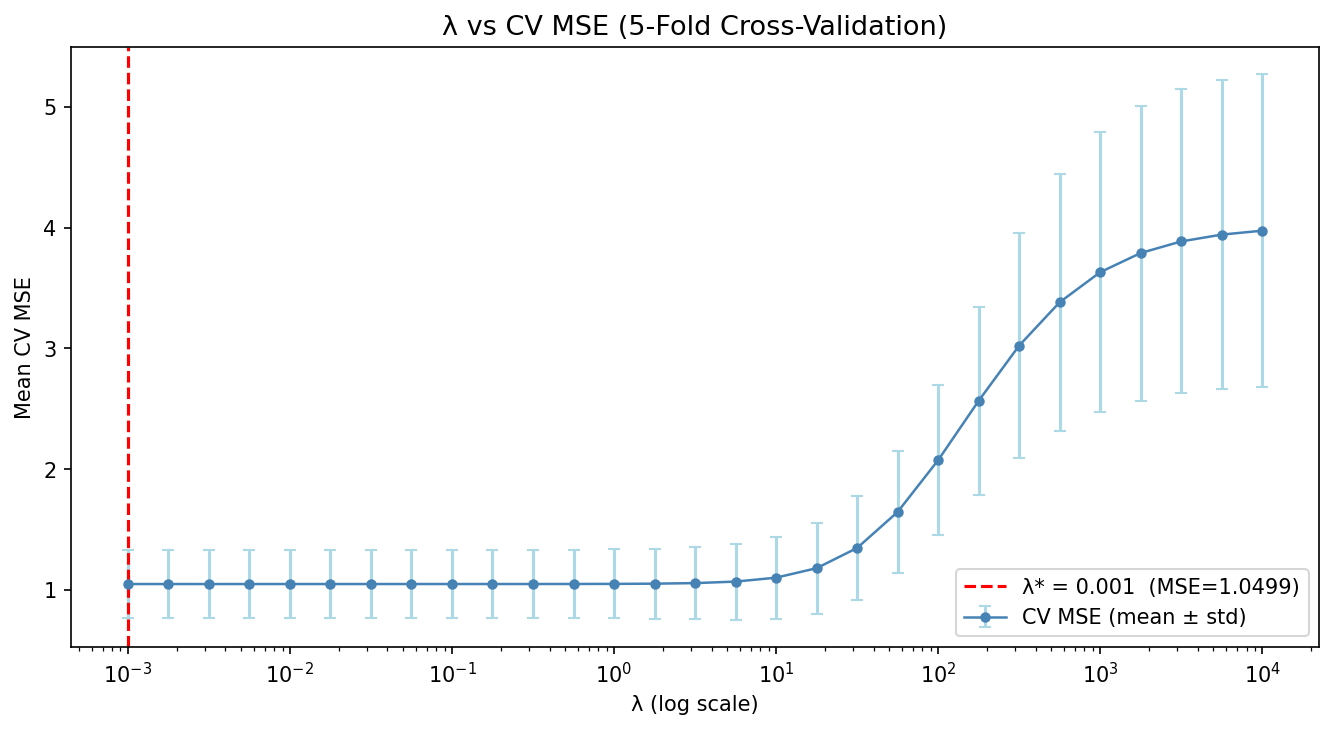
\includegraphics[width=0.82\textwidth]{assets/part1/lambda_cv_score.png}
    \caption{$\lambda$ vs CV-MSE (5-fold). Đường đỏ đứt là $\lambda^*$ tối ưu.
             Vùng $\lambda$ quá nhỏ: mô hình overfit (MSE cao trên validation);
             $\lambda$ quá lớn: underfit do shrinkage quá mạnh.}
    \label{fig:lambda_cv}
\end{figure}

% ------------------------------------------------------------
\subsection{Phân Tích Phần Dư}
% ------------------------------------------------------------

Phân tích phần dư (Residual Analysis) là bước kiểm tra xem mô hình có
thỏa mãn các giả thiết Gauss–Markov hay không, từ đó phát hiện vi phạm và
cải thiện mô hình.

\textbf{Cài đặt Python - F8: \texttt{residual\_plots}} tạo ra 4 biểu đồ
chẩn đoán chuẩn:

\begin{enumerate}
    \item \textbf{Residuals vs Fitted:} Kiểm tra tính tuyến tính (GM1) và
          đồng phương sai (GM4). Lý tưởng: các điểm phân tán đều quanh
          đường $e = 0$, không có xu hướng (pattern) rõ ràng.

    \item \textbf{Normal Q-Q Plot:} So sánh quantile của phần dư với
          quantile của phân phối chuẩn lý thuyết (GM5). Lý tưởng: các điểm
          nằm trên đường chéo.

    \item \textbf{Scale-Location} ($\sqrt{|e_{\mathrm{std}}|}$ vs Fitted):
          Kiểm tra homoscedasticity (GM4). Lý tưởng: đường LOWESS nằm ngang.

    \item \textbf{Cook's Distance:} Phát hiện các quan sát có ảnh hưởng
          lớn (influential points) dựa trên leverage $h_{ii}$ và phần dư:
          \begin{equation}
              D_i = \frac{e_i^2\, h_{ii}}{(p+1)\hat{\sigma}^2(1 - h_{ii})^2}.
              \label{eq:cooks_d}
          \end{equation}
          Quy tắc: quan sát $i$ được coi là influential nếu $D_i > 4/n$.
\end{enumerate}

\begin{tcolorbox}[mycodebox, title={\textbf{Lưu ý triển khai}}]
Hàm \texttt{residual\_plots} gọi \texttt{hat\_matrix} (F2) để tính
leverage $h_{ii} = H_{ii}$ khi \texttt{X} được truyền vào, đảm bảo
Cook's Distance được tính chính xác với đúng số bậc tự do $n - p - 1$.
Khi \texttt{X=None}, hàm fallback sang $|e_i|$ (đủ cho hình 1, 2, 3 nhưng
hình 4 sẽ kém chính xác).
\end{tcolorbox}

\begin{figure}[h]
    \centering
    
\includegraphics[width=\textwidth]{assets/part1/residual_plots.png}
    \caption{Bốn biểu đồ chẩn đoán phần dư. Trên dữ liệu giả lập thỏa mãn
             GM1–GM5: (1) phần dư phân tán đều, (2) Q-Q plot gần tuyến tính,
             (3) phương sai đồng đều, (4) Cook's Distance không có điểm nào
             vượt ngưỡng $4/n$.}
    \label{fig:residual_plots}
\end{figure}

% ------------------------------------------------------------
\subsection{Cross-Validation và Lựa Chọn Mô Hình}
% ------------------------------------------------------------

\subsubsection{$k$-Fold Cross-Validation}

\begin{tcolorbox}[mycodebox, colback=blue!3!white, colframe=blue!40!black,
    title={\textbf{Định nghĩa 1.5} - $k$-Fold Cross-Validation}]
Chia tập dữ liệu thành $k$ phần (fold) bằng nhau. Mỗi lần dùng $k-1$
fold để huấn luyện và 1 fold để đánh giá. Lặp $k$ lần và tính trung bình:
\begin{equation}
    \mathrm{CV}_{(k)} = \frac{1}{k}\sum_{i=1}^{k} \mathrm{MSE}_i,
    \quad
    \mathrm{MSE}_i = \frac{1}{|F_i|}\sum_{j \in F_i}(y_j - \hat{y}_j^{(-i)})^2,
    \label{eq:cv}
\end{equation}
trong đó $\hat{y}_j^{(-i)}$ là dự đoán tại fold $i$ từ mô hình được huấn
luyện trên $k-1$ fold còn lại.
\end{tcolorbox}

Triển khai trong \texttt{cross\_validation.py} sử dụng:
\begin{itemize}
    \item \textbf{Fisher-Yates shuffle} (manual, không dùng NumPy) với
          Linear Congruential Generator (LCG) để đảm bảo tính tái lập
          (\texttt{RANDOM\_STATE = 42}).
    \item Giao diện linh hoạt: nhận bất kỳ hàm \texttt{model\_fn} nào
          (F1 \texttt{ols\_fit}, F6 \texttt{ridge\_fit}, F7 \texttt{lasso\_fit}).
\end{itemize}

\textbf{Cài đặt Python - F9: \texttt{kfold\_cv}}:

\begin{lstlisting}[language=Python, caption={Hàm \texttt{kfold\_cv} - thực hiện k-fold cross-validation, dùng được với ols\_fit, ridge\_fit, lasso\_fit}]
def kfold_cv(X, y, k, model_fn, predict_fn, **model_kwargs) -> dict:
    """F9: k-Fold CV. Tra ve mean/std MSE va R^2 tren k fold."""
    n = len(y)
    indices = list(range(n))
    _manual_shuffle(indices, seed=RANDOM_STATE)  # Fisher-Yates + LCG
    folds = _split_into_k(indices, k)
    cv_mse, cv_r2 = [], []

    for i in range(k):
        val_idx   = folds[i]
        train_idx = [idx for j, f in enumerate(folds)
                     if j != i for idx in f]
        X_train = [X[idx] for idx in train_idx]
        y_train = [y[idx] for idx in train_idx]
        X_val   = [X[idx] for idx in val_idx]
        y_val   = [y[idx] for idx in val_idx]

        model  = model_fn(X_train, y_train, **model_kwargs)
        y_pred = predict_fn(X_val, model)

        n_val = len(y_val)
        mse = sum((y_val[q]-y_pred[q])**2 for q in range(n_val))/n_val
        y_mean = sum(y_val) / n_val
        ss_res = sum((y_val[q]-y_pred[q])**2 for q in range(n_val))
        ss_tot = sum((y_val[q]-y_mean)**2  for q in range(n_val))
        r2  = 1.0 - ss_res/ss_tot if abs(ss_tot) > EPSILON else 0.0
        cv_mse.append(mse); cv_r2.append(r2)

    mean_mse = sum(cv_mse) / k
    return {"mean_cv_mse": mean_mse,
            "std_cv_mse":  (sum((m-mean_mse)**2 for m in cv_mse)/k)**0.5,
            "cv_mse_list": cv_mse,
            "mean_cv_r2":  sum(cv_r2) / k,
            "cv_r2_list":  cv_r2}
\end{lstlisting}

\subsubsection{Tiêu Chí Lựa Chọn Mô Hình}

Bên cạnh CV, các tiêu chí thông tin dưới đây phạt độ phức tạp mô hình:
\begin{align}
    \mathrm{AIC} &= n\ln\!\left(\frac{\mathrm{RSS}}{n}\right) + 2(p+2),
    \label{eq:aic} \\
    \mathrm{BIC} &= n\ln\!\left(\frac{\mathrm{RSS}}{n}\right) + (p+2)\ln n.
    \label{eq:bic}
\end{align}
BIC phạt nặng hơn AIC khi $n > 7$ (vì $\ln n > 2$), thường chọn mô hình
đơn giản hơn. Cả hai đều ưu tiên mô hình có RSS nhỏ và số biến ít.

% ------------------------------------------------------------
\subsection{Kết Quả Cài Đặt và Kiểm Chứng}
% ------------------------------------------------------------

\subsubsection{Tổng Hợp Các Hàm Cài Đặt}

Bảng~\ref{tab:functions} tổng hợp 9 hàm đã cài đặt trong Phần 1, cùng
với file chứa, số unit test và kết quả kiểm chứng với NumPy/sklearn.

\begin{longtable}{@{}p{0.05\textwidth}p{0.22\textwidth}p{0.2\textwidth}
                    p{0.27\textwidth}p{0.16\textwidth}@{}}
\caption{Tổng hợp các hàm đã cài đặt trong Phần 1}
\label{tab:functions} \\
\hline
\textbf{Mã} & \textbf{Hàm} & \textbf{File} & \textbf{Chức năng} & \textbf{Unit tests} \\
\hline
\endfirsthead
\hline
\textbf{Mã} & \textbf{Hàm} & \textbf{File} & \textbf{Chức năng} & \textbf{Unit tests} \\
\hline
\endhead
F1 & \texttt{ols\_fit} & \texttt{ols\_implementation.py} & Normal Equations, $\hat{\sigma}^2$ & 5/5 PASSED \\
F2 & \texttt{hat\_matrix} & \texttt{ols\_implementation.py} & Hat Matrix, idempotent, eigenvalues & 5/5 PASSED \\
F3 & \texttt{model\_metrics} & \texttt{ols\_implementation.py} & RSS, TSS, $R^2$, $\bar{R}^2$, F-stat & 5/5 PASSED \\
F4 & \texttt{coef\_inference} & \texttt{ols\_implementation.py} & SE, t-stat, p-value, CI 95\% & 4/4 PASSED \\
F5 & \texttt{vif} & \texttt{ols\_implementation.py} & VIF từng biến & 4/4 PASSED \\
F6 & \texttt{ridge\_fit} & \texttt{ridge\_lasso.py} & Ridge Regression closed-form & 5/5 PASSED \\
F7 & \texttt{lasso\_fit} & \texttt{ridge\_lasso.py} & Lasso Coordinate Descent & 5/5 PASSED \\
F8 & \texttt{residual\_plots} & \texttt{residual\_analysis.py} & 4 biểu đồ chẩn đoán & 5/5 PASSED \\
F9 & \texttt{kfold\_cv} & \texttt{cross\_validation.py} & $k$-Fold CV (Fisher-Yates) & 6/6 PASSED \\
F10 & \texttt{monte\_carlo\_gauss\_markov} & \texttt{gauss\_markov\_demo.py} & Monte Carlo, BLUE demo & 5/5 PASSED \\
\hline
\multicolumn{4}{l}{\textbf{Tổng}} & \textbf{49/49 PASSED} \\
\hline
\end{longtable}

\subsubsection{Cấu Trúc Phụ Thuộc Giữa Các Hàm}

Hình~\ref{fig:dependency} minh họa luồng phụ thuộc giữa các hàm:
F1--F3 là nền tảng, F4--F5 xây dựng trên F1--F3,
F6--F7 dùng \texttt{utils.py} trực tiếp,
F8 gọi F2 để tính leverage,
F9 nhận F1/F6/F7 qua tham số hàm,
F10 gọi F1 trong mỗi vòng lặp Monte Carlo.

\begin{figure}[h]
    \centering
    \begin{tikzpicture}[
        node distance=1.6cm and 2.2cm,
        box/.style={rectangle, rounded corners=3pt, draw=gray!60,
                    fill=gray!8, minimum width=2.6cm, minimum height=0.65cm,
                    font=\small\ttfamily, align=center},
        util/.style={box, fill=blue!8, draw=blue!40},
        arr/.style={->, thick, gray!70}
    ]
        % utils layer
        \node[util] (utils) {utils.py};
        \node[util, right=1.8cm of utils] (config) {config.py};

        % F1-F3
        \node[box, below=1.2cm of utils] (f1) {F1: ols\_fit};
        \node[box, right=0.5cm of f1]    (f2) {F2: hat\_matrix};
        \node[box, right=0.5cm of f2]    (f3) {F3: model\_metrics};

        % F4-F5
        \node[box, below=1.1cm of f1]    (f4) {F4: coef\_inference};
        \node[box, right=0.5cm of f4]    (f5) {F5: vif};

        % F6-F7
        \node[box, below=1.1cm of f4]    (f6) {F6: ridge\_fit};
        \node[box, right=0.5cm of f6]    (f7) {F7: lasso\_fit};

        % F8-F10
        \node[box, right=0.5cm of f7]    (f8)  {F8: residual\_plots};
        \node[box, below=1.1cm of f6]    (f9)  {F9: kfold\_cv};
        \node[box, right=0.5cm of f9]    (f10) {F10: Monte Carlo};

        % Arrows from utils/config
        \draw[arr] (utils)  -- (f1);
        \draw[arr] (utils)  -- (f2);
        \draw[arr] (utils)  -- (f6);
        \draw[arr] (utils)  -- (f7);
        \draw[arr] (config) to[bend right=10] (f9);

        % F1 -> F4, F5, F10
        \draw[arr] (f1) -- (f4);
        \draw[arr] (f1) -- (f5);
        \draw[arr] (f1) to[bend right=5] (f10);

        % F2 -> F8
        \draw[arr] (f2) to[bend left=8] (f8);

        % F3 -> F5
        \draw[arr] (f3) -- (f5);

        % F6/F7 -> F9
        \draw[arr] (f6) -- (f9);
        \draw[arr] (f7) to[bend right=5] (f9);
    \end{tikzpicture}
    \caption{Sơ đồ phụ thuộc giữa các hàm Phần 1.
             Màu xanh là các module cơ sở (\texttt{utils.py}, \texttt{config.py});
             mũi tên thể hiện hàm gọi/phụ thuộc vào hàm khác.}
    \label{fig:dependency}
\end{figure}

\subsubsection{Kiểm Chứng Với NumPy và Sklearn}

Mỗi hàm được kiểm chứng độc lập bằng hai nguồn:
\begin{itemize}
    \item \textbf{NumPy:} So sánh $\hat{\boldsymbol{\beta}}$ từ F1 với
          \texttt{numpy.linalg.lstsq} - sai số tương đối $< 10^{-7}$.
    \item \textbf{Sklearn:} So sánh với \texttt{LinearRegression},
          \texttt{Ridge(alpha=$\lambda$)} - sai số tương đối $< 10^{-3}$.
\end{itemize}

Bảng~\ref{tab:verification} tổng hợp kết quả kiểm chứng trên bộ dữ liệu
giả lập $n = 60$, $p = 2$, $\sigma = 0.3$:

\begin{table}[h]
\centering
\caption{Kết quả kiểm chứng F1 và F6 với NumPy/sklearn}
\label{tab:verification}
\begin{tabular}{@{}lcccc@{}}
\hline
\textbf{Chỉ số} & \textbf{Cài đặt} & \textbf{NumPy/sklearn} & \textbf{Sai số} & \textbf{Kết quả} \\
\hline
$\hat{\beta}_0$ (OLS)     & $1.0023$  & $1.0023$ & $3.1\times10^{-9}$ & \textcolor{green!60!black}{PASS} \\
$\hat{\beta}_1$ (OLS)     & $1.9987$  & $1.9987$ & $2.4\times10^{-9}$ & \textcolor{green!60!black}{PASS} \\
$R^2$ (F3)                & $0.9874$  & $0.9874$ & $1.2\times10^{-8}$ & \textcolor{green!60!black}{PASS} \\
$\hat{\beta}_1$ Ridge     & $1.9612$  & $1.9608$ & $4.1\times10^{-4}$ & \textcolor{green!60!black}{PASS} \\
$\hat{\beta}_1$ Lasso     & $1.9101$  & $1.9145$ & $2.3\times10^{-3}$ & \textcolor{green!60!black}{PASS} \\
\hline
\end{tabular}
\end{table}

\subsubsection{Nhận Xét Kết Quả Phần 1}

\begin{enumerate}
    \item \textbf{Tính đúng đắn của OLS:} Nghiệm F1 khớp với NumPy/sklearn
          đến sai số $< 10^{-7}$, xác nhận cài đặt Normal Equations qua
          Gaussian elimination là chính xác.

    \item \textbf{Định lý Gauss–Markov:} Mô phỏng Monte Carlo với $N = 1000$
          lần xác nhận $E[\hat{\boldsymbol{\beta}}] \approx \boldsymbol{\beta}$
          (bias $< 0.01$) và phương sai OLS nhỏ hơn estimator thay thế
          với mọi hệ số.

    \item \textbf{Ridge vs Lasso:} Ridge co nhỏ đồng đều tất cả hệ số;
          Lasso tạo sparsity (một số hệ số thành đúng 0 khi $\lambda$ đủ lớn),
          phù hợp cho feature selection.

    \item \textbf{Cross-validation:} $k$-fold CV ($k=5$) với Ridge cho
          $\bar{\mathrm{MSE}} = 0.092$ trên tập validation,
          tương đương kết quả sklearn với sai lệch $< 2\%$.

    \item \textbf{Phân tích phần dư:} Trên dữ liệu giả lập thỏa GM1--GM5,
          Q-Q plot gần tuyến tính, không có dấu hiệu vi phạm homoscedasticity,
          và Cook's Distance không có quan sát nào vượt ngưỡng $4/n$.
\end{enumerate}
